% Options for packages loaded elsewhere
\PassOptionsToPackage{unicode}{hyperref}
\PassOptionsToPackage{hyphens}{url}
%
\documentclass[
  ignorenonframetext,
  aspectratio=169]{beamer}
\usepackage{pgfpages}
\setbeamertemplate{caption}[numbered]
\setbeamertemplate{caption label separator}{: }
\setbeamercolor{caption name}{fg=normal text.fg}
\beamertemplatenavigationsymbolsempty
% Prevent slide breaks in the middle of a paragraph
\widowpenalties 1 10000
\raggedbottom
\setbeamertemplate{part page}{
  \centering
  \begin{beamercolorbox}[sep=16pt,center]{part title}
    \usebeamerfont{part title}\insertpart\par
  \end{beamercolorbox}
}
\setbeamertemplate{section page}{
  \centering
  \begin{beamercolorbox}[sep=12pt,center]{part title}
    \usebeamerfont{section title}\insertsection\par
  \end{beamercolorbox}
}
\setbeamertemplate{subsection page}{
  \centering
  \begin{beamercolorbox}[sep=8pt,center]{part title}
    \usebeamerfont{subsection title}\insertsubsection\par
  \end{beamercolorbox}
}
\AtBeginPart{
  \frame{\partpage}
}
\AtBeginSection{
  \ifbibliography
  \else
    \frame{\sectionpage}
  \fi
}
\AtBeginSubsection{
  \frame{\subsectionpage}
}
\usepackage{lmodern}
\usepackage{amssymb,amsmath}
\usepackage{ifxetex,ifluatex}
\ifnum 0\ifxetex 1\fi\ifluatex 1\fi=0 % if pdftex
  \usepackage[T1]{fontenc}
  \usepackage[utf8]{inputenc}
  \usepackage{textcomp} % provide euro and other symbols
\else % if luatex or xetex
  \usepackage{unicode-math}
  \defaultfontfeatures{Scale=MatchLowercase}
  \defaultfontfeatures[\rmfamily]{Ligatures=TeX,Scale=1}
\fi
% Use upquote if available, for straight quotes in verbatim environments
\IfFileExists{upquote.sty}{\usepackage{upquote}}{}
\IfFileExists{microtype.sty}{% use microtype if available
  \usepackage[]{microtype}
  \UseMicrotypeSet[protrusion]{basicmath} % disable protrusion for tt fonts
}{}
\makeatletter
\@ifundefined{KOMAClassName}{% if non-KOMA class
  \IfFileExists{parskip.sty}{%
    \usepackage{parskip}
  }{% else
    \setlength{\parindent}{0pt}
    \setlength{\parskip}{6pt plus 2pt minus 1pt}}
}{% if KOMA class
  \KOMAoptions{parskip=half}}
\makeatother
\usepackage{xcolor}
\IfFileExists{xurl.sty}{\usepackage{xurl}}{} % add URL line breaks if available
\IfFileExists{bookmark.sty}{\usepackage{bookmark}}{\usepackage{hyperref}}
\hypersetup{
  pdftitle={Reporte de Ventas MBM Servicio de Envíos},
  hidelinks,
  pdfcreator={LaTeX via pandoc}}
\urlstyle{same} % disable monospaced font for URLs
\newif\ifbibliography
\setlength{\emergencystretch}{3em} % prevent overfull lines
\providecommand{\tightlist}{%
  \setlength{\itemsep}{0pt}\setlength{\parskip}{0pt}}
\setcounter{secnumdepth}{-\maxdimen} % remove section numbering
\setbeamertemplate{navigation symbols}{} %remove nav bar

\usepackage{booktabs}
\usepackage{graphicx}


\usetheme{metropolis}
\setsansfont{Open Sans}

\newenvironment<>{varblock}[2][.95\textwidth]{%
  \setlength{\textwidth}{#1}
  \begin{actionenv}#3%
    \def\insertblocktitle{#2}%
    \par%
    \usebeamertemplate{block begin}}
  {\par%
    \usebeamertemplate{block end}%
  \end{actionenv}}
  
\usepackage{array}
\ifluatex
  \usepackage{selnolig}  % disable illegal ligatures
\fi

\title{Reporte de Ventas MBM Servicio de Envíos}
\author{}
\date{\vspace{-2.5em}}

\begin{document}
\frame{\titlepage}

\begin{frame}{Resumen Mensual al 2020-10-17}
\protect\hypertarget{resumen-mensual-al-2020-10-17}{}
\begin{columns}[T]
    \begin{column}{0.25\textwidth} %first column
    Mejores Clientes
    \scriptsize

\begin{tabular}{>{\raggedright\arraybackslash}p{0.8in}rl}
\toprule
cliente & wh & ganancias\\
\midrule
Alfonso Campillo & 2 & \$ 670.24\\
Berardo D'antonio & 8 & \$ 156.45\\
Adrian Aguirre & 2 & \$ 121.80\\
Astrid Querales & 7 & \$ 119.24\\
Nestor Guerrero & 3 & \$  99.98\\
\addlinespace
Isai Albert & 6 & \$  70.70\\
Yerse Renginfo & 1 & \$  61.20\\
Vanessa Zambrano (Tu Vida Organica) & 2 & \$  49.30\\
Enmanuel Millans & 2 & \$  49.20\\
Juan Macias (Socio) & 5 & \$  46.08\\
\bottomrule
\end{tabular}
    \normalsize
    \end{column}
    \begin{column}{0.45\textwidth} %first column
    Mes Corriente
    \scriptsize

\begin{tabular}{>{\raggedright\arraybackslash}p{0.5in}rlrr}
\toprule
Envio & Wh & Ganancias & Lb & Ft\\
\midrule
AEREO & 143 & \$ 1,376.70 & 776 & 0.00\\
MARITIMO & 23 & \$ 1,070.71 & 0 & 273.68\\
\bottomrule
\end{tabular}
    \normalsize
    \end{column}
\end{columns}
\end{frame}

\begin{frame}{Resumen}
\protect\hypertarget{resumen}{}
\begin{columns}[T]
    \begin{column}{0.90\textwidth} %first column
    Resumen de Ventas Consolidado
    \scriptsize

\begin{tabular}{>{\raggedright\arraybackslash}p{0.9in}rlrr}
\toprule
Mes & Warehouse & Ganancias & Libras & Feet\\
\midrule
Diciembre-2019 & 53 & \$   660.20 & 358 & 39.846\\
Enero-2020 & 67 & \$   538.80 & 179 & 68.683\\
Febrero-2020 & 56 & \$   456.39 & 258 & 38.966\\
Marzo-2020 & 72 & \$   517.22 & 240 & 50.633\\
Abril-2020 & 105 & \$ 1,069.80 & 538 & 48.198\\
\addlinespace
Mayo-2020 & 242 & \$ 1,364.35 & 787 & 34.066\\
Junio-2020 & 320 & \$ 1,766.03 & 1039 & 93.034\\
Julio-2020 & 469 & \$ 3,286.17 & 1778 & 193.724\\
Agosto-2020 & 351 & \$ 2,356.04 & 1051 & 118.215\\
Septiembre-2020 & 319 & \$ 2,567.22 & 1133 & 116.847\\
\addlinespace
Octubre-2020 & 166 & \$ 2,447.41 & 776 & 273.680\\
\bottomrule
\end{tabular}
    \normalsize
    \end{column}
\end{columns}
\end{frame}

\begin{frame}{Anual}
\protect\hypertarget{anual}{}
\begin{columns}[T]
    \begin{column}{0.25\textwidth} %first column
    Mejores Clientes
    \scriptsize

\begin{tabular}{>{\raggedright\arraybackslash}p{0.8in}rl}
\toprule
cliente & wh & ganancias\\
\midrule
Berardo D'antonio & 131 & \$ 1,280.00\\
Isai Albert & 83 & \$ 1,101.19\\
Adrian Aguirre & 92 & \$ 1,081.65\\
Alfonso Campillo & 48 & \$ 1,034.20\\
Reinaldo Valdes & 156 & \$ 1,022.69\\
\addlinespace
Nestor Guerrero & 19 & \$   656.01\\
Maria Vielma (Cliente Doterra) & 96 & \$   561.41\\
Vanessa Zambrano (Tu Vida Organica) & 53 & \$   535.50\\
Karen Gallo (Cliente Doterra) & 85 & \$   517.54\\
Ana Cristina Perez (Cliente Doterra) & 35 & \$   493.40\\
\bottomrule
\end{tabular}
    \normalsize
    \end{column}
    \begin{column}{0.45\textwidth} %first column
    Últimos 5 Meses
    \scriptsize

\begin{tabular}{>{\raggedright\arraybackslash}p{0.5in}lrlrr}
\toprule
Mes & Envio & Wh & Ganancias & Lb & Ft\\
\midrule
Jun-2020 & AEREO & 262 & \$ 1,511.15 & 1039 & 0.000\\
Jun-2020 & MARITIMO & 58 & \$   254.88 & 0 & 93.034\\
Jul-2020 & AEREO & 369 & \$ 2,569.20 & 1778 & 0.000\\
Jul-2020 & MARITIMO & 100 & \$   716.97 & 0 & 193.724\\
Ago-2020 & AEREO & 299 & \$ 1,653.71 & 1051 & 0.000\\
\addlinespace
Ago-2020 & MARITIMO & 52 & \$   702.33 & 0 & 118.215\\
Sep-2020 & AEREO & 260 & \$ 1,926.75 & 1133 & 0.000\\
Sep-2020 & MARITIMO & 59 & \$   640.47 & 0 & 116.847\\
Oct-2020 & AEREO & 143 & \$ 1,376.70 & 776 & 0.000\\
Oct-2020 & MARITIMO & 23 & \$ 1,070.71 & 0 & 273.680\\
\bottomrule
\end{tabular}
    \normalsize
    \end{column}
\end{columns}
\end{frame}

\begin{frame}{Gráfico al 2020-10-17 Aeréo y Marítimo}
\protect\hypertarget{gruxe1fico-al-2020-10-17-aeruxe9o-y-maruxedtimo}{}
\begin{columns}[T]
    \begin{column}{0.90\textwidth} %first column
    \scriptsize

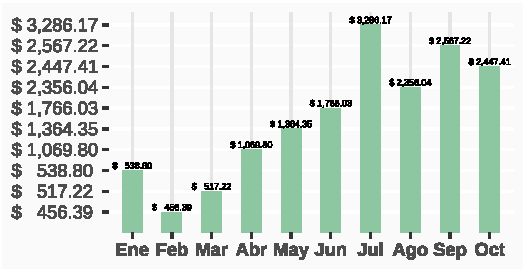
\includegraphics[width=\textwidth]{Reporte MBM_files/figure-beamer/unnamed-chunk-10-1} 
    \normalsize
    \end{column}
\end{columns}
\end{frame}

\begin{frame}{Gráfico al 2020-10-17 Aeréo}
\protect\hypertarget{gruxe1fico-al-2020-10-17-aeruxe9o}{}
\begin{columns}[T]
    \begin{column}{0.90\textwidth} %first column
    \scriptsize

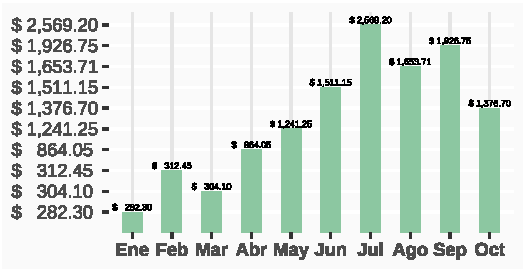
\includegraphics[width=\textwidth]{Reporte MBM_files/figure-beamer/unnamed-chunk-12-1} 
    \normalsize
    \end{column}
\end{columns}
\end{frame}

\begin{frame}{Gráfico al 2020-10-17 Marítimo}
\protect\hypertarget{gruxe1fico-al-2020-10-17-maruxedtimo}{}
\begin{columns}[T]
    \begin{column}{0.90\textwidth} %first column
    \scriptsize

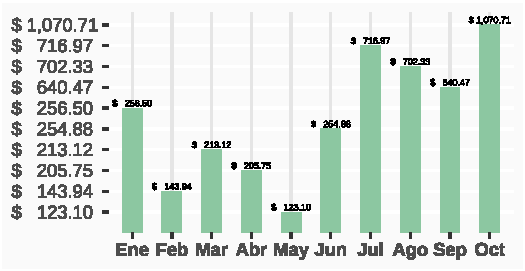
\includegraphics[width=\textwidth]{Reporte MBM_files/figure-beamer/unnamed-chunk-14-1} 
    \normalsize
    \end{column}
\end{columns}
\end{frame}

\end{document}
